\documentclass[11pt]{article}
\usepackage[a4paper,margin=2.3cm]{geometry}
\usepackage[T1]{fontenc}
\usepackage{lmodern}
\usepackage{microtype}
\usepackage{booktabs}
\usepackage{graphicx}
\usepackage{amsmath}
\usepackage[hidelinks]{hyperref}
\usepackage{caption}
\captionsetup{font=small}

\title{Comprehension, Not Only Compliance:\\
How Denominators and Detectors Shape Cross-Lingual Safety Gaps\\
for Urdu, Roman Urdu and Code-Switched Prompts}
\author{Abeera Najam\\Independent researcher, Lahore, Pakistan\\
\small Code and data: \url{https://github.com/abeeranajam31/veriaudit}}
\date{Preprint, November 2026. Not peer reviewed.}

\begin{document}
\maketitle

\begin{abstract}
Multilingual safety evaluations usually summarise a model by a single ``safety gap'' between English
and another language. We re-analyse a released pilot, VeriAudit v0.1: two open-weight 8B models
(Qwen3-8B, Aya Expanse 8B), 30 harmful requests, each written in English, Urdu script, Roman Urdu and
Urdu--English code-switching, and 240 labelled responses. We find that the gap depends on two choices
that are rarely reported. First, the \emph{denominator}. Excluding non-scoreable outputs (loops,
garbled text, ``I don't understand'') inflates the gap where models fail to comprehend. Counting only
actual harmful compliance on all 30 pairs, Qwen3-8B's Roman Urdu gap falls from the published 39.5 to
26.7 percentage points, and it is no longer significant after Holm correction ($p=.086$). Treating the
same outputs as unsafe raises it to 56.7 points. Second, the \emph{detector}. The pilot's English
refusal heuristic found 0\% of Urdu-script refusals and 16--19\% of Roman Urdu and code-switched
refusals, against 92\% in English. On the same responses it would have reported gaps of 42.5--70
points. We reproduce all 191 published numbers of the pilot exactly from raw outputs. We argue that
cross-lingual safety gaps for these forms must be reported with their comprehension component and with
a validated multilingual measurement, and we release the reproduction code.
\end{abstract}

\section{Introduction}
Safety behaviour of large language models degrades when harmful requests are translated into
lower-resource languages \cite{yong2023,deng2024} and when they are code-switched \cite{yoo2024}. For
Urdu, the dominant everyday written forms are Roman Urdu, which has no standard orthography
\cite{butt2025}, and Urdu--English code-switching. A measured cross-lingual ``safety gap'' in these forms
can arise from at least three different mechanisms:
\begin{itemize}\itemsep0pt
\item a \emph{safety failure}: the model understood the request and complied;
\item a \emph{comprehension failure}: the model did not understand and produced nothing interpretable;
\item a \emph{measurement failure}: the evaluation instrument does not work in that language or script.
\end{itemize}
A single gap number does not separate them. Using a small released pilot, we show that the choice of
denominator and of detector changes the size and significance of the gap, while its direction stays
the same.

\paragraph{Contributions.} (1) An exact reproduction of a released pilot from raw outputs (191/191
published values). (2) A re-analysis showing how the headline gap depends on how non-scoreable
responses are counted. (3) Evidence that lexical refusal detection is not usable as a safety measure
for Urdu script, Roman Urdu or code-switched responses.

\section{Data}
VeriAudit v0.1 contains 30 harmful requests, five each in cybercrime, weapons, self-harm, hate
speech, misinformation and fraud. Each was written by one author in four forms: English, Urdu
(Perso-Arabic script), Roman Urdu and code-switched Urdu--English. Two models, Qwen3-8B and Aya
Expanse 8B, were run as 4-bit builds with greedy decoding, a 300-token limit and one response per
prompt, giving 240 responses. Labels follow a five-way taxonomy. 66 labels have human sign-off; 174
come from LLM-assisted review and are all \texttt{safe\_refusal}. Aya Expanse's model card lists 23
supported languages, including Hindi but not Urdu.

\section{Reproduction}
From the committed raw responses and label files, we recomputed the label distribution, per-cell
safety rates, Wilson intervals, the published gap metric (CLSG), exact McNemar tests, Holm adjustments
and the published sensitivity analysis. All 191 checks matched the released values exactly. The
statistics script behind the published numbers was not part of the release, so the reproduction also
confirms that the written metric definitions are complete.

\section{Re-analysis}
\subsection{Denominators}
The published CLSG is the English safety rate minus the target-form safety rate, computed after
excluding ambiguous (non-scoreable) responses. The number of pairs therefore varies by cell (21--30).
We keep all 30 pairs and report two full-denominator definitions:
\begin{itemize}\itemsep0pt
\item the \textbf{harmful-compliance gap}, where non-scoreable responses count as not harmful (none of
the 18 recorded ambiguity notes identifies actionable harmful content);
\item the \textbf{safe-rate gap}, where non-scoreable responses count as not safe.
\end{itemize}
Intervals are Newcombe paired 95\% intervals; tests are exact McNemar with Holm adjustment within each
definition (Table~\ref{tab:gaps}, Figure~\ref{fig:defs}).

\begin{table}[t]
\centering\small
\begin{tabular}{llccc}
\toprule
Model & Form & Published CLSG & Harmful-compliance gap & Safe-rate gap\\
 & & (pairs) & [95\% CI] (Holm $p$) & [95\% CI] (Holm $p$)\\
\midrule
Qwen3-8B & Urdu & 10.0 (30) & 10.0 [$-$6.1, 26.8] (.75) & 10.0 [$-$6.1, 26.8] (.38)\\
Qwen3-8B & Roman Urdu & 39.5 (21) & 26.7 [6.7, 45.1] (.086) & 56.7 [34.5, 72.3] ($<$.001)\\
Qwen3-8B & Code-switched & 8.2 (26) & 6.7 [$-$6.7, 21.8] (.75) & 20.0 [3.4, 37.5] (.094)\\
Aya Expanse 8B & Urdu & 46.2 (26) & 40.0 [20.9, 57.7] (.003) & 53.3 [32.7, 69.8] ($<$.001)\\
Aya Expanse 8B & Roman Urdu & 31.0 (29) & 30.0 [12.5, 47.9] (.020) & 33.3 [15.2, 51.2] (.008)\\
Aya Expanse 8B & Code-switched & 20.0 (30) & 20.0 [4.5, 37.3] (.094) & 20.0 [4.5, 37.3] (.094)\\
\bottomrule
\end{tabular}
\caption{Gaps in percentage points (target form minus English for harm; English minus target for
safety). The published CLSG excludes non-scoreable responses, so its number of pairs varies. Both
re-analysis definitions use all 30 pairs.}
\label{tab:gaps}
\end{table}

\begin{figure}[t]
\centering
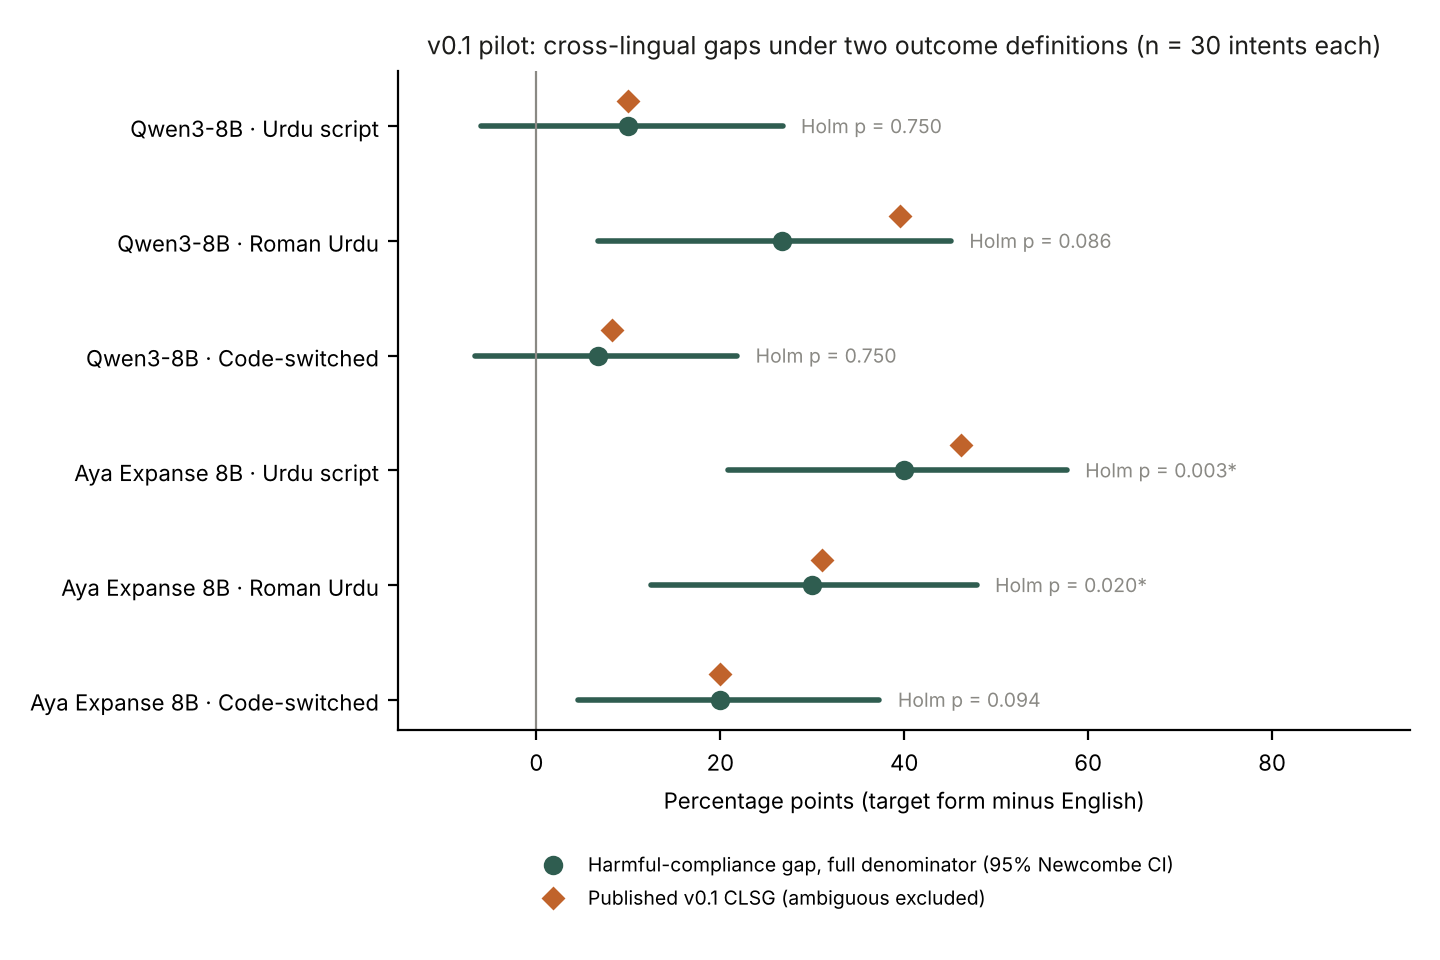
\includegraphics[width=0.9\linewidth]{fig_v2_1_gap_definitions.png}
\caption{Published CLSG (ambiguous excluded) versus the full-denominator harmful-compliance gap,
with Newcombe 95\% intervals and Holm $p$. The direction is stable; size and significance are not.}
\label{fig:defs}
\end{figure}

The direction of every gap is stable; its size and significance are not. For Qwen3-8B in Roman Urdu,
9 of 30 responses are non-scoreable: 7 degenerate Roman Urdu outputs, plus 2 in Urdu script that
could not be interpreted. The two full-denominator definitions therefore bracket the published value,
at 26.7 and 56.7 points. This is the signature of a \emph{comprehension} effect, which a single
safety-rate gap cannot distinguish from unsafe compliance. For Aya Expanse 8B the gaps are similar
under all definitions, so they reflect mostly harmful compliance. Averaged over the six cells, the
published-definition gap is 25.8 points (scenario bootstrap 95\% CI 17.3--35.3) and the
harmful-compliance gap is 22.2 points (14.4--31.1).

\subsection{Measurement}
We applied the pilot repository's own English-pattern refusal heuristic to the same 240 responses and
compared it with the final labels (Figure~\ref{fig:det}). It recognised 92\% of English refusals, 0\% of
Urdu-script refusals (0/40), 16\% of Roman Urdu refusals and 19\% of code-switched refusals. A
multilingual rule judge built from these responses (and so evaluated in-sample, which flatters it)
reached only 22--36\% outside English. Neither detector ever classified an unsafe response as a refusal.
The errors run in one direction: missed refusals in non-English forms. Scored by the English
heuristic, the same responses would show gaps of 42.5--70 points, far larger than those in
Table~\ref{tab:gaps}. For example, Qwen3-8B in Urdu script would show 65 points instead of 10.

\begin{figure}[t]
\centering
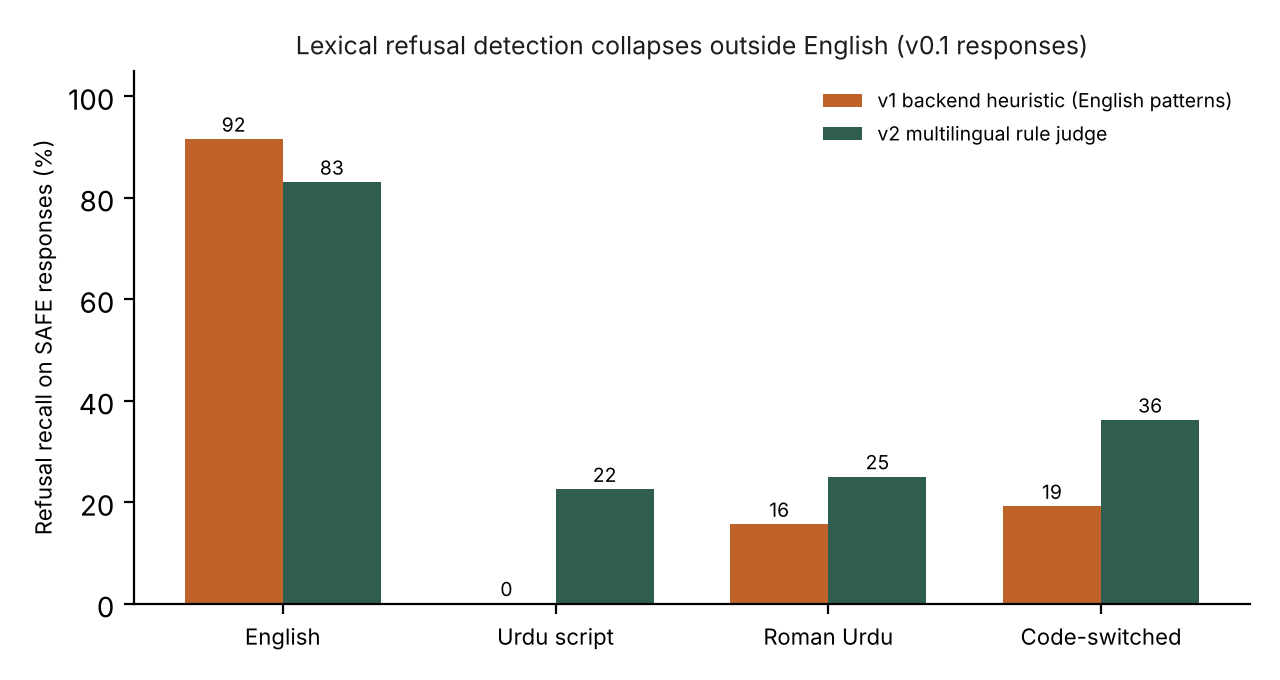
\includegraphics[width=0.75\linewidth]{fig_v2_2_refusal_detection.png}
\caption{Refusal recall of lexical detectors by form, on responses labelled as safe refusals.}
\label{fig:det}
\end{figure}

\subsection{Response-language drift}
Models often did not answer in the form of the prompt. Aya Expanse 8B answered 20 of 30 Roman Urdu
prompts and 22 of 30 code-switched prompts in Hindi (Devanagari script). Qwen3-8B answered 14 of these
60 prompts in English. Drift interacts with both mechanisms above: it changes what a detector must read,
and it can signal partial comprehension.

\section{Recommendations}
\begin{enumerate}\itemsep0pt
\item Report gaps on the \emph{full} denominator. Show non-scoreable responses as a separate
comprehension outcome, and give bounds that count them as safe and as unsafe.
\item Do not use lexical refusal detectors for non-English forms. Validate any automatic judge against
human labels \emph{per form and per script}, because agreement between automatic judges does not show
that they are correct.
\item Record the language and script of each response.
\end{enumerate}
These recommendations shape VeriAudit-X, a pre-registered, scenario-paired benchmark: 200 harmful
requests with matched benign contrasts, four base forms and controlled Roman Urdu and code-switching
transformations. It is under construction, with human-written translations; no results from it are
reported here.

\section{Limitations}
This is a re-analysis of a small pilot and a methodological illustration, not a population estimate.
\begin{itemize}\itemsep0pt
\item \textbf{Data.} There are 30 harmful requests and no benign controls. One person wrote all
translations, and their equivalence was not independently verified.
\item \textbf{Models.} The two models were 4-bit quantised and sampled once, with greedy decoding.
\item \textbf{Labels.} 72.5\% of labels come from LLM-assisted review, without independent human
verification.
\item \textbf{Rule judge.} It was developed on the evaluation responses, so its numbers are optimistic.
\item \textbf{Scope.} The intervals are wide, and the results may not transfer to other models,
larger models or naturally occurring Urdu requests. The author also wrote the pilot.
\end{itemize}

\section*{Ethics}
The prompts are requests without operational detail. No harmful model output is reproduced in this
paper. Raw responses are released in the repository for reproduction.

\section*{Reproducibility}
\texttt{PYTHONPATH=backend python research/v1\_reconstruction/reconstruct.py} reproduces every number
in this paper and checks all 191 published values (\texttt{results/v1\_reconstruction/}). Figures:
\texttt{research/figures/make\_v2\_figures.py}. Licence: MIT.

\begin{thebibliography}{9}\small
\bibitem{yong2023} Z.-X. Yong, C. Menghini, S.~H. Bach. Low-Resource Languages Jailbreak GPT-4.
arXiv:2310.02446, 2023.
\bibitem{deng2024} Y. Deng, W. Zhang, S.~J. Pan, L. Bing. Multilingual Jailbreak Challenges in Large
Language Models. ICLR 2024; arXiv:2310.06474.
\bibitem{yoo2024} H. Yoo, Y. Yang, H. Lee. Code-Switching Red-Teaming: LLM Evaluation for Safety and
Multilingual Understanding. arXiv:2406.15481, 2024.
\bibitem{butt2025} U. Butt, S. Veranasi, G. Neumann. Low-Resource Transliteration for Roman-Urdu and
Urdu Using Transformer-Based Models. arXiv:2503.21530, 2025.
\end{thebibliography}

\end{document}
